% ============================================================
%  main_zh.tex  —  中文碩士論文
%  國立臺灣大學管理學院財務金融研究所
%  編譯指令：xelatex main_zh（建議執行兩次以正確產生目錄）
% ============================================================
\documentclass[12pt, a4paper, oneside]{ctexbook}

% ── 字型設定 ─────────────────────────────────────────────────
% 中文：標楷體。在 Mac/Windows 上請改用：\setCJKmainfont{標楷體}
% 本 Linux 系統使用 AR PL UKai TW 作為等效替代
\setCJKmainfont{AR PL UKai TW}
\setCJKsansfont{AR PL UKai TW}
\setCJKmonofont{AR PL UKai TW}
% 英文：Times New Roman。在已安裝 TNR 的系統上請改用：\setmainfont{Times New Roman}
\usepackage{fontspec}
\setmainfont{TeX Gyre Termes}

% ── 章節標題格式 ─────────────────────────────────────────────
\ctexset{
  chapter/name     = {第,章},
  chapter/number   = \chinese{chapter},
  chapter/format   = \centering\Large\bfseries,
  section/format   = \large\bfseries,
  subsection/format = \normalsize\bfseries,
}

% ── 頁面版型（上 3cm、下 2cm、左右各 3cm）────────────────────
\usepackage{geometry}
\geometry{a4paper, top=3cm, bottom=2cm, left=3cm, right=3cm}

% ── 行距：1.5 倍 ─────────────────────────────────────────────
\usepackage{setspace}
\onehalfspacing

% ── 頁碼置中於頁底 ───────────────────────────────────────────
\pagestyle{plain}

% ── 台大校徽浮水印（每頁右上角）──────────────────────────────
% ── 共用前言（表格、數學、圖、自訂指令等） ───────────────────
% ============================================================
%  preamble.tex  —  shared by main.tex (English) and main_zh.tex (Chinese)
% ============================================================

% --- Tables --------------------------------------------------
\usepackage{booktabs}       % \toprule \midrule \bottomrule
\usepackage{multirow}       % \multirow{n}{*}{text}
\usepackage{makecell}       % line breaks inside cells
\usepackage{tabularx}       % auto-width columns

% --- Figures -------------------------------------------------
\usepackage{graphicx}
\usepackage{caption}        % \captionof for non-floating tables
\usepackage{subcaption}     % \begin{subfigure}

% --- Math ----------------------------------------------------
\usepackage{amsmath}
% \usepackage{amssymb}
\usepackage{bm}             % bold math \bm{}

% --- Numbers & Units -----------------------------------------
\usepackage{siunitx}
\usepackage{enumitem}
\sisetup{
  round-mode      = places,
  round-precision = 3,
  table-format    = 1.3,
}

% --- Typography ----------------------------------------------
\usepackage{microtype}      % better line breaking

% --- Diagrams ------------------------------------------------
\usepackage{tikz}
\usetikzlibrary{shapes.geometric, arrows.meta, positioning, fit, backgrounds}

% --- Bibliography --------------------------------------------
% natbib provides \citet{} and \citep{}
\usepackage[round,authoryear]{natbib}

% --- Cross-references ----------------------------------------
\usepackage{hyperref}
\usepackage{cleveref}       % \cref{} \Cref{}

% --- Fonts ----------------------------------------
\usepackage{amsfonts}

% ============================================================
%  Terminology Glossary (EN → ZH)
%  Cross-Sectional           橫截面
%  Ranking Loss              排序損失
%  Gradient Accumulation     梯度累積
%  Ensemble                  集成
%  Feature Configuration     特徵組合
%  Walk-forward              滾動前向
%  Sharpe Ratio              夏普比率
%  Long-Short Portfolio      多空投資組合
%  Variable Selection Net    變數選擇網路
%  Gated Residual Network    門控殘差網路
%  Temporal Fusion Transformer  時序融合轉換器
%  Cross-Asset Attention     跨資產注意力
% ============================================================

% --- Custom commands -----------------------------------------
\newcommand{\SR}{\mathrm{SR}}          % Sharpe Ratio abbreviation
\newcommand{\NW}{\mathrm{NW}}          % Newey–West
\newcommand{\btau}{\bm{\tau}}
\newcommand{\bx}{\bm{x}}
\newcommand{\by}{\bm{y}}
\newcommand{\cL}{\mathcal{L}}
\newcommand{\cF}{\mathcal{F}}
\newcommand{\R}{\mathbb{R}}

% Bold table header helper
\renewcommand{\thead}[1]{\textbf{#1}}

% Significance stars
\newcommand{\sig}[1]{%
  \ifnum#1=3 $^{***}$\fi
  \ifnum#1=2 $^{**}$\fi
  \ifnum#1=1 $^{*}$\fi
}



% NTU logo watermark
% NTU watermark following mediaic/NTU_MS_Thesis.
% Source settings: vector NTU seal, absolute scale 40%, opacity 20%,
% behind page, watermark center 2.5 cm from top and right.
\usepackage{eso-pic}

\newcommand{\NTUWatermark}{%
  \AddToShipoutPictureBG{%
    \put(\LenToUnit{\dimexpr\paperwidth-2.5cm-50.4bp\relax},
         \LenToUnit{\dimexpr\paperheight-2.5cm-50.4bp\relax}){%
      \begin{tikzpicture}
        \node[anchor=south west, inner sep=0pt, opacity=0.20]
          {
\includegraphics[width=100.8bp]{NTU_logo_gray}};%
      \end{tikzpicture}%
    }%
  }%
}

\NTUWatermark


% ── hyperref 設定（需在 preamble 載入後調整） ─────────────────
\hypersetup{
  colorlinks = true,
  linkcolor  = black,
  citecolor  = black,
  urlcolor   = black,
}

% ============================================================
\begin{document}

%% ─────────────────────────────────────────────────────────────
%% 前置部分（頁碼：羅馬數字）
%% ─────────────────────────────────────────────────────────────
\frontmatter

% ── 封面 ─────────────────────────────────────────────────────
\begin{titlepage}
\begin{singlespace}
\centering
\vspace*{1cm}

{\fontsize{18}{27}\selectfont 國立臺灣大學管理學院財務金融研究所\par
                               碩士論文\par}
{\fontsize{14}{21}\selectfont Department of Finance\par
                               College of Management\par}
{\fontsize{16}{24}\selectfont National Taiwan University\par
                               Master's Thesis\par}

\vfill

{\fontsize{18}{27}\selectfont 利用排序正規化深度學習進行\\
                               加密貨幣橫截面報酬預測\par}
\vspace{6pt}
{\fontsize{18}{27}\selectfont Cross-Sectional Cryptocurrency Return Prediction\\
                               via Rank-Normalized Deep Learning\par}

\vfill

{\fontsize{18}{27}\selectfont 陳\quad 芃\par
                               Peng Chen\par}

\vfill

{\fontsize{18}{27}\selectfont 指導教授：蕭湛東 博士\par
                               Advisor: Dr.\ Lawrence Hsiao\par}

\vfill

{\fontsize{18}{27}\selectfont 中華民國 115 年 6 月\par
                               June 2026\par}

\vspace{3cm}
\end{singlespace}
\end{titlepage}

% ── 論文口試委員審定書 ────────────────────────────────────────
\chapter*{論文口試委員審定書}
\addcontentsline{toc}{chapter}{論文口試委員審定書}
\thispagestyle{plain}

\vspace{1cm}
\noindent 本論文係陳芃君（學號 R12723071）在國立臺灣大學財務金融研究所完成之碩士學位論文，
於民國\underline{\hspace{2em}}年\underline{\hspace{2em}}月\underline{\hspace{2em}}日承下列考試委員審查通過及口試及格，特此證明。

\vspace{3cm}
\noindent 口試委員：

\vspace{1.5cm}
\hspace{4cm}\underline{\hspace{8cm}}（指導教授）

\vspace{1.2cm}
\hspace{4cm}\underline{\hspace{8cm}}

\vspace{1.2cm}
\hspace{4cm}\underline{\hspace{8cm}}

\vspace{1.2cm}
\hspace{4cm}\underline{\hspace{8cm}}

\vspace{2cm}
\noindent 系主任、所長\underline{\hspace{8cm}}

% ── 謝辭 ─────────────────────────────────────────────────────
\chapter*{謝辭}
\addcontentsline{toc}{chapter}{謝辭}
\thispagestyle{plain}

\noindent 謹向指導教授蕭湛東博士致以最深切的感謝，感謝在研究過程中給予的悉心指導、
寶貴建議與持續鼓勵。

% ── 中文摘要 ─────────────────────────────────────────────────
\chapter*{中文摘要}
\addcontentsline{toc}{chapter}{中文摘要}
\thispagestyle{plain}

% 對應英文：sections/01_abstract.tex
% TODO: 翻譯後請同步更新英文版的修改

預測下週哪些加密貨幣將超越同類資產，本質上是一個橫截面排序問題，
然而過去的研究普遍採用不適合排序目標的時間序列損失函數。
本文證明，這種目標函數與評估標準之間的不匹配，
是深度學習模型在此類任務中表現遜於普通最小二乘法（OLS）的主要原因。

本文的核心方法貢獻，在於將 ListNet 排序損失的目標訊號從原始報酬替換為
橫截面排名百分位：每個資產依其在當週橫截面中的排名，被賦予介於 $[0, 1]$
的監督信號（Poh 等人，2021），無論當週報酬的絕對波動幅度為何，
每個資產對損失梯度的貢獻均等。

本文在一個涵蓋 324 週 $\times$ 86 種加密貨幣的週資料面板上，
評估三種深度學習架構——具有跨資產注意力的 LSTM、採用完整變數選擇網路的時序融合轉換器（TFT），
以及全新設計的橫截面門控網路（CS-Gated）——並與六種傳統基準模型進行比較。

最佳模型 CS-Gated（以鏈上特徵訓練）在年化夏普比率上達到 2.75（等權多空組合），
而 LSTM 搭配川普社群媒體與 ETF 資金流特徵則達到 2.13。
整體結果顯示，深度學習在正確的排序損失下可與傳統方法競爭，
但不同模型對不同訊號型態各有優勢，隨機森林在高維資訊集下仍具強勁表現。
消融研究（ablation study）確認，排名正規化搭配梯度累積，
是促成績效改善的關鍵機制。


\vspace{1em}
\noindent\textbf{關鍵詞：}加密貨幣、橫截面預測、排序損失、時序融合轉換器、機器學習

% ── 英文摘要 ─────────────────────────────────────────────────
\chapter*{Abstract}
\addcontentsline{toc}{chapter}{Abstract}
\thispagestyle{plain}

Predicting which cryptocurrencies will outperform in the following week
is fundamentally a cross-sectional ranking task, yet prior work has
applied time-series loss functions ill-suited to ranking objectives.
We demonstrate that this mismatch is the primary reason deep learning
models often underperform ordinary least squares in standard configurations.
%
Our key methodological contribution is the use of rank-percentile
normalized targets with ListNet ranking loss: instead of softmax-weighting
raw returns, we assign each asset its cross-sectional rank percentile as
the supervision signal, eliminating scale sensitivity across heterogeneous
volatility regimes.
%
We evaluate three deep learning architectures—LSTM with cross-asset
attention, a corrected Temporal Fusion Transformer (TFT), and a novel
CrossSectionalGatedNet (CS-Gated)—against six traditional baselines on
a panel of 324 weeks $\times$ 86 cryptocurrencies.
%
The best model, CS-Gated trained on on-chain features, achieves an
annualized Sharpe ratio of 2.75 (equal-weight long-short portfolio),
while LSTM with Trump social media and ETF flow features reaches 2.13.
The results show that deep learning becomes competitive once the ranking
objective is specified correctly, although different architectures remain
best suited to different signal types.
An ablation study confirms that rank normalization together with gradient
accumulation, rather than architectural novelty alone, drives the improvement.


\vspace{1em}
\noindent\textbf{Keywords:} cryptocurrency, cross-sectional prediction, ranking loss,
temporal fusion transformer, machine learning

% ── 目錄、圖目錄、表目錄 ─────────────────────────────────────
\tableofcontents
\listoffigures
\listoftables

%% ─────────────────────────────────────────────────────────────
%% 論文正文（頁碼：阿拉伯數字）
%% ─────────────────────────────────────────────────────────────
\mainmatter

\chapter{導論}
\label{sec:intro}
% 對應英文：sections/02_introduction.tex

加密貨幣市場已由 \citet{nakamoto2008bitcoin} 所提出的單一去中心化資產，
發展為一個涵蓋眾多代幣、鏈上經濟機制與政策曝險的異質資產市場。
\citet{liu2022cryptocurrency} 指出，加密貨幣的橫截面報酬具有自身的風險因子結構，
其中動量與規模溢酬雖與股票市場相似，卻在形成機制與市場微結構上呈現明顯差異。
在此背景下，預測哪些代幣會在下一週相對於其他資產表現更佳，
本質上並非單純的時間序列點預測問題，而是一個需要比較資產彼此相對強弱的橫截面排序問題。
對於一個涵蓋 86 種積極交易代幣、同時包含價格、鏈上、總體、政策訊號與 ETF 資金流資料的宇宙而言，
模型不僅需要整合異質特徵，還必須學會一種「相對報酬」而非「絕對報酬」的預測概念。

\paragraph{既有文獻與研究缺口。}
\citet{gu2020empirical} 是機器學習資產定價文獻中的代表性研究，
指出在特徵集充足且模型容量受到適當正則化時，
樹模型與神經網路能夠系統性超越線性基準。
\citet{freyberger2020dissecting} 進一步說明，
資產特徵之間的非線性交互作用本身就攜帶顯著的額外預測力。
這些發現自然引導出一個問題：
若橫截面特徵在股票市場已具有高度解釋力，
那麼在波動更大、資訊來源更雜訊化的加密貨幣市場中，
機器學習是否同樣能有效地從橫截面訊號中擷取可交易的排序資訊？

加密貨幣文獻已經證明此市場具備可預測性，但對模型機制的結論並不一致。
\citet{cakici2024crypto_ml} 發現，
加密貨幣橫截面報酬的可預測性確實存在，
但模型複雜度所帶來的邊際收益可能有限；
\citet{filippou2024crypto_ml} 則顯示，
在涵蓋動量、網路活動、技術指標與投資人關注的豐富特徵集合下，
非線性模型可產生顯著的樣本外預測與經濟價值。
這些研究共同說明，問題不在於加密貨幣是否可預測，
而在於如何讓模型以正確的方式學習可比較、可交易的橫截面信號。

本文認為，深度學習模型在此類任務中經常表現不如預期，
關鍵原因並不一定是架構不足，而是目標函數與評估標準之間的錯配。
當標準 ListNet 損失 \citep{cao2007learning} 直接以原始下週報酬作為 softmax 目標時，
不同週次的目標分布會因波動幅度不同而產生截然不同的尖銳度。
在高波動週次，少數極端資產主導梯度；
在平靜週次，目標分布又接近均勻，導致梯度訊號過弱。
\citet{poh2021building} 在股票橫截面研究中已指出這個問題，
並建議以排名百分位取代原始報酬作為 ListNet 的監督訊號。
本文將此想法延伸至加密貨幣市場，
因其跨資產波動率差異更大，故目標尺度不一致的問題更加嚴重。

\paragraph{資料面向的研究動機。}
除了損失函數外，本文的另一個動機來自資料來源的擴充。
\citet{cong2021tokenomics} 與 \citet{liu2022cryptocurrency} 指出，
鏈上指標如 NVT、MVRV 與網路活動資料，
可反映加密貨幣與股票市場截然不同的基本面結構。
另一方面，傳統金融文獻早已證明替代資料的重要性：
\citet{tetlock2007giving} 顯示媒體語調對股票短期價格有預測力，
\citet{bollen2011twitter} 則發現 Twitter 情緒可領先部分市場變動。
在加密貨幣市場中，\citet{maitre2025social} 進一步指出，
社群媒體注意力與橫截面報酬之間存在可檢測的關聯。
因此，若研究只停留在價格與鏈上資料，可能低估與政策訊號或敘事熱度相關的報酬來源。

本文特別引入兩類過去較少在同一框架下整合的結構性資料。
第一類是川普在 Truth Social 與 X 上的發文特徵，
用以捕捉高影響力政策行為者在關稅與加密監管議題上的公開表態；
第二類是 Farside Investors 自 2024 年 1 月現貨比特幣 ETF 核准後所提供的細粒度資金流資料
\citep{bitcoin_etf_farside}，
可將 ETF 總流量拆解為 Grayscale 存量資金贖回與排除 GBTC/ETHE 後的新增資金流入。
在我們所掌握的文獻中，
將鏈上基本面、政策相關社群媒體訊號與 ETF 結構性資金流
同時放入橫截面排序模型中進行比較，仍屬相對少見。

\paragraph{架構設計上的考量。}
在模型架構方面，本文同時檢驗三種不同的歸納偏誤。
LSTM \citep{hochreiter1997long,fischer2018lstm_finance}
擅長從有限回看窗口中擷取時序依賴，是金融時間序列中穩健的基準模型。
TFT \citep{lim2021temporal} 則透過變數選擇網路與注意力機制，
強調可解釋性與對異質輸入的處理能力。
然而，\citet{gu2020empirical} 的結論也提醒我們：
若真正有效的是橫截面當期特徵，那麼複雜的時序編碼器未必必要。
基於這一點，本文另外提出不含時序編碼器的 CrossSectionalGatedNet，
藉由門控殘差網路與跨資產注意力，直接檢驗「純橫截面架構是否已足以完成排序任務」。

\paragraph{研究貢獻。}
基於上述研究缺口，本文有四項主要貢獻：
\begin{enumerate}
  \item \textbf{排名正規化的 ListNet 目標。}
        依循 \citet{poh2021building}，
        以橫截面排名百分位 $\in [0, 1]$ 取代原始報酬作為 softmax 目標，
        降低不同市場環境下的目標尺度不一致問題。
  \item \textbf{梯度累積。}
        透過將有效橫截面批次大小由每步 86 個資產提升至
        $86 \times 4 = 344$ 個資產，
        進一步穩定排序損失的梯度方向。
  \item \textbf{橫截面門控網路（CrossSectionalGatedNet）。}
        本文提出一個不含時序編碼器的架構，
        由多層 GRN 與跨資產注意力構成，
        用以檢驗橫截面結構本身是否足以支撐加密貨幣的排序任務。
  \item \textbf{修正後的 TFT 變數選擇網路。}
        我們以每變數共享的 GRN 取代過度簡化的輕量 VSN，
        使 TFT 的實作更貼近 \citet{lim2021temporal} 的原始規格，
        並提升特徵選擇的穩定性。
\end{enumerate}

\paragraph{章節架構。}
第~\ref{sec:related}~節回顧相關文獻，
並說明本文與既有加密貨幣機器學習研究的差異。
第~\ref{sec:data}~節介紹資料面板、特徵來源與偏誤控制。
第~\ref{sec:method}~節形式化排序損失與模型架構。
第~\ref{sec:experiments}~節說明超參數設定與六組資訊集設計。
第~\ref{sec:results}~節報告跨模型比較結果。
第~\ref{sec:analysis}~節進一步討論消融研究、Granger 因果檢定、子期間穩健性與集成效果。
第~\ref{sec:conclusion}~節總結研究發現與限制。


\chapter{相關研究}
\label{sec:related}
% 對應英文：sections/03_related_work.tex

\section{橫截面報酬預測的機器學習方法}

\citet{gu2020empirical} 為機器學習橫截面資產定價提供了經典基礎，
指出在特徵集豐富的情況下，
樹模型與神經網路均能超越傳統線性模型，
而真正的預測力往往來自特徵之間的非線性交互作用，而非單一指標本身。
\citet{freyberger2020dissecting} 亦從非參數角度證實，
當資產特徵之間存在複雜交互項時，
線性模型對平均報酬的近似能力有限。
這組文獻的重要啟示在於：
若橫截面特徵已經足夠豐富，模型的關鍵任務不一定是建構更長的時序記憶，
而是學會如何比較當期不同資產之間的相對位置。

在加密貨幣市場中，\citet{liu2022cryptocurrency} 建立了共同風險因子的基本框架，
顯示動量與規模等效果在加密資產中確實存在，但其形成方式與股票市場不同。
更直接相關的是 \citet{cakici2024crypto_ml} 與 \citet{filippou2024crypto_ml}：
前者以多種機器學習方法研究加密貨幣橫截面報酬，
指出報酬可預測性大致來自少數簡單特徵，模型複雜度的邊際報酬有限；
後者則發現，在納入網路活動、動量、技術指標與投資人關注等資料後，
非線性模型可產生顯著的樣本外預測力與經濟價值。
這些研究說明，加密貨幣市場的可預測性並非不存在，
而是取決於模型如何對異質特徵進行整合與排序。
本文的 CS-Gated 架構，正是沿著這條脈絡，
直接測試「僅依賴當期橫截面訊號」是否已足以生成高品質排序。

\section{金融領域的學習排序方法}

學習排序文獻 \citep{cao2007learning} 為橫截面投資組合建構提供了自然的理論基礎。
與直接預測報酬值不同，排序方法的目標是讓高分資產在橫截面上穩定地排在低分資產之前，
因此更貼近多空投資組合的實務需求。
\citet{poh2021building} 是與本文最直接相關的先驅工作：
他們指出，若直接將原始報酬放入 ListNet 的 softmax 目標，
會因不同期別的報酬尺度差異而造成訓練不穩定；
改用橫截面排名百分位後，模型在股票橫截面上的排序績效顯著改善。

本文完整承襲其核心想法，但將其置於波動更高的加密貨幣市場中重新檢驗。
相較於股票市場，加密貨幣之間的波動率差距更大，
同一週內不同資產的報酬分布也更容易出現厚尾與極端值。
因此，目標函數尺度不一致在本研究設定下更加嚴重，
也使排名正規化更具有方法論上的必要性。
此外，本文再加入梯度累積，以改善每一步 ListNet 梯度所依賴的橫截面經驗分布品質，
藉此將排序方法從「可訓練」進一步推向「穩定可重現」。

\section{時序深度學習架構}

LSTM \citep{hochreiter1997long,fischer2018lstm_finance} 長期被視為金融時間序列中的穩健基準，
其優勢在於能以相對節制的參數量整合有限回看窗口中的局部時序依賴。
對於社群媒體發文量、ETF 資金流或其他具有事件延續性的訊號而言，
LSTM 能有效捕捉短期序列模式，
因此仍是本文不可或缺的比較基準。

另一方面，TFT \citep{lim2021temporal} 結合變數選擇網路、LSTM 編碼器與多頭注意力，
強調對異質輸入的可解釋整合。
相較一般 Transformer 架構 \citep{vaswani2017attention}，
TFT 更適合處理同時包含靜態與時變特徵的金融場景。
然而，TFT 的優勢通常伴隨較高模型容量與較高訓練不穩定性，
因此本文特別修正其變數選擇網路，使其更接近原始規格，
並與 LSTM 及純橫截面架構進行並列比較。
這樣的設計使我們得以回答一個更具研究價值的問題：
究竟是「時序編碼能力」本身帶來改善，
還是「正確的損失函數與特徵配置」才是績效差異的主要來源。

\section{替代資料來源}

替代資料在金融預測中的應用已相當廣泛。
\citet{tetlock2007giving} 證明媒體內容可影響股票短期報酬，
\citet{bollen2011twitter} 則顯示 Twitter 心情指標能在一定程度上領先市場變動。
在加密貨幣領域，\citet{maitre2025social} 進一步指出，
社群媒體注意力與加密貨幣橫截面報酬存在顯著關聯，
代表文字與敘事熱度已成為不可忽視的市場資訊來源。

本文使用的川普社群媒體特徵與上述文獻不同，
並非衡量整體市場情緒，而是捕捉單一高影響力政策人物的訊號。
這種設計的意義在於將「政策敘事」視為可量化的結構性衝擊來源，
而非單純的雜訊情緒代理變數。
同時，ETF 資金流資料則補上鏈上資料無法直接觀察到的機構需求面。
自 2024 年 1 月現貨比特幣 ETF 核准後，
\citet{bitcoin_etf_farside} 所提供的細粒度流量資料，
使研究者得以區分 Grayscale 存量資金贖回與新增資金流入，
這對於理解事件後的供需結構具有獨特價值。
本文將這兩類資料與價格、技術、鏈上特徵放入同一排序框架，
目的不只是追求更高績效，
更是希望辨識不同資料型態對不同模型架構的適配性。

\section{統計推斷方法}

金融機器學習研究若只報告樣本外績效而不處理序列相關性與非常態問題，
容易高估策略的統計可信度。
因此，本文採用 Newey--West
\citep{newey1987simple,newey1994automatic}
異方差與自相關一致（HAC）$t$ 統計量，
並使用 Politis 與 Romano \citep{politis1994stationary}
提出的定態區塊自助法來構建夏普比率的信賴區間。
這些方法並不直接提高模型績效，
但可避免將短樣本、集中的市場行情或偶然極端報酬誤判為穩健結論，
對於僅有 49 週測試期的本文而言尤其重要。


\chapter{資料}
\label{sec:data}
% 對應英文：sections/04_data.tex

\section{面板概覽}

本研究的資料集為一個平衡面板，涵蓋 $T = 324$ 個週度觀測值
（2020-01-05 至 2026-03-15），共 $N = 86$ 種加密貨幣。
原始資料檔保留 53 個特徵欄位；依據最終 v6 實驗設定，
本文在六組資訊集中實際使用其中 42 個模型輸入特徵，
其餘欄位保留於資料檔中供後續擴充，不列入本版實證比較。
橫截面固定為 2026 年 3 月市值排名前 86 的代幣，
尚未上市資產在對應週次的缺失值以 $-99.99$ 標記，
並在損失計算與評估時加以遮罩。

\section{特徵類別}

表~\ref{tab:features} 彙整了本文實際納入模型的 42 個特徵，
可概分為七個群組。
這樣的分組設計反映了本文的核心研究問題：
不同資料型態是否需要不同的模型歸納偏誤，才能轉化為穩健的橫截面排序績效。

\begin{table}[t]
\centering
\caption{本文實際納入模型之特徵類別。$M_g$ 表示第 $g$ 類特徵數。}
\label{tab:features}
\small
\begin{tabular}{llc}
\toprule
\thead{類別} & \thead{代表特徵} & \thead{$M_g$} \\
\midrule
價格與動量         & 1/4/12/26/52 週報酬                         & 5  \\
技術指標           & RSI、布林帶、ATR、OBV、成交量比率          & 6  \\
鏈上指標           & 活躍地址數、交易數、NVT、交易所凈流量、MVRV & 5  \\
總體與市場情緒     & 恐懼貪婪指數、S\&P 500、DXY、VIX、金銀報酬  & 11 \\
ETF 與 Polymarket  & BTC/ETH ETF 流量、Polymarket BTC 機率      & 6  \\
川普社群媒體       & 發文數、大寫比例、關稅分數、加密分數、情緒  & 5  \\
Farside ETF 細粒度 & GBTC、BTC ex-GBTC、ETHE、ETH ex-ETHE       & 4  \\
\midrule
合計               &                                              & 42 \\
\bottomrule
\end{tabular}
\end{table}

價格與技術指標提供最直接的市場行為訊號，
鏈上變數則反映代幣網路的使用與估值狀態；
總體變數捕捉美元流動性與風險偏好的共同環境，
而社群媒體與 ETF 資金流特徵則代表具有事件性與制度性特徵的替代資料。
這種由「慢變基本面」到「快變事件訊號」的結構差異，
也是本文後續比較橫截面模型與時序模型的重要基礎。

\section{資料切割}
\label{sec:data:splits}

我們按時間順序將面板切割為訓練集（70\%，第 0--226 週）、
驗證集（15\%，第 227--274 週）與測試集（15\%，第 275--323 週，共 49 週）。
所有超參數均在驗證集上選擇，測試集僅用於最終一次評估，
以避免在模型設計過程中反覆使用測試期資訊。

\section{前瞻偏差分析}
\label{sec:data:lookahead}

本文特別檢查三種可能的前瞻偏差來源。
第一，所有特徵均以 52 週滾動 Z 分數進行標準化；
在第 $t$ 週，每個特徵只使用區間 $[t-51, t]$ 的均值與標準差，
不會引用未來週次資料。
這種作法與 \citet{gu2020empirical} 的處理精神一致，
即使包含當期值，其在 52 週窗口中的權重也僅約為 $1/52$，
屬金融時間序列研究中的常見作法。

第二，川普社群媒體特徵是以每週結束前可觀察到的貼文內容所構建：
發文數、大寫比例、關稅分數、加密分數與情緒指標，
均僅使用該週內已發布的 Truth Social 與 X 貼文。
第三，ETF 資金流特徵由每日資料聚合為週頻後，再於當週做滾動標準化，
因此亦不包含未來資訊。
綜合而言，本文的主要風險不在於 look-ahead bias，
而在於資料覆蓋率與市場結構變動所造成的估計不穩定。

\section{存活偏差}
\label{sec:data:survival}

本文的 86 種資產係依 2026 年 3 月的市值排名固定選定，
因此不可避免地帶有前瞻性的存活偏差：
若某些 2020 年至 2026 年間曾活躍、但後續衰退或下架的代幣未被納入，
則樣本中的平均報酬與流動性條件可能較實際市場更為樂觀。
這個限制會影響絕對績效水準的解讀，
特別是多空策略在小型、脆弱代幣上的可交易性評估。

然而，存活偏差對本文的跨模型比較不致構成致命問題。
原因在於所有模型皆面對相同的資產宇宙、相同的切割方式與相同的資訊集，
因此比較結果仍可用來判斷不同損失函數與模型架構的相對優劣。
換言之，本文的結論應更被解讀為
「在給定樣本宇宙下，何種方法較適合處理加密貨幣橫截面排序問題」，
而非對整體加密貨幣市場可投資性做無條件外推。


\chapter{方法論}
\label{sec:method}
% 對應英文：sections/05_methodology.tex

\section{問題形式化}

設 $\bx_{i,t} \in \R^M$ 為資產 $i$ 在第 $t$ 週的特徵向量，
$r_{i,t+1}$ 為下一週的實現報酬。
我們的目標是學習一個評分函數 $f_\theta : \R^M \to \R$，
使得當 $r_{i,t+1} > r_{j,t+1}$ 時，$f_\theta(\bx_{i,t}) > f_\theta(\bx_{j,t})$
對第 $t$ 週橫截面中所有 $(i,j)$ 配對成立。
我們在每週依 $f_\theta(\bx_{\cdot,t})$ 做多頂部十分位、放空底部十分位，
構建多空投資組合。

\section{排名正規化的 ListNet 損失}
\label{sec:method:loss}

標準 ListNet（Cao 等人，2007）透過帶溫度參數 $\tau$ 的 softmax
將分數與目標轉換為概率分布：
\begin{equation}
  P_i = \frac{\exp(s_i / \tau)}{\sum_j \exp(s_j / \tau)}, \quad
  Q_i = \frac{\exp(y_i / \tau)}{\sum_j \exp(y_j / \tau)},
\end{equation}
其中 $s_i = f_\theta(\bx_{i,t})$，$y_i = r_{i,t+1}$。
損失為交叉熵 $\cL = -\sum_i Q_i \log P_i$。

\paragraph{原始報酬的問題。}
當 $y_i = r_{i,t+1}$ 時，在波動性大的週次，目標分布 $Q$ 會被少數極端報酬的資產主導；
在平靜的週次則接近均勻分布。
這種尺度敏感性在加密貨幣報酬的異質波動率環境中使訓練不穩定。

\paragraph{排名百分位正規化。}
依循 Poh 等人（2021），以橫截面排名百分位取代原始報酬：
\begin{equation}
  \tilde{y}_{i,t} = \frac{\mathrm{rank}(r_{i,t+1};\, \{r_{j,t+1}\}_{j=1}^N) - 1}{N - 1}
  \in [0, 1],
\end{equation}
使表現最佳的資產始終獲得 $\tilde{y} = 1$，最差的始終獲得 $\tilde{y} = 0$，
與當週報酬的絕對幅度無關。
在上述公式中以 $\tilde{y}_{i,t}$ 取代 $y_i$，可確保每個資產對目標分布的貢獻均等，
損失梯度對橫截面波動率縮放不變。

\section{LSTM 架構}
\label{sec:method:lstm}

LSTM 模型先對每個資產的 $L$ 步特徵歷史進行編碼，再執行跨資產比較。
給定特徵序列 $X_i = (\bx_{i,t-L+1}, \dots, \bx_{i,t}) \in \R^{L \times M}$，
前向傳播步驟如下：

\begin{enumerate}[nosep]
  \item \textbf{輸入投影與位置編碼。}
        $H = \mathrm{Dropout}(W_\text{in} X_i) + P$，
        其中 $W_\text{in} \in \R^{M \times d}$，
        $P \in \R^{L \times d}$ 為可學習的位置嵌入（$d=64$）。

  \item \textbf{LSTM 編碼器。}
        單層 LSTM 處理 $H$，輸出最終隱藏狀態 $h_i \in \R^d$。

  \item \textbf{資產嵌入。}
        加入可學習的資產嵌入 $e_i \in \R^d$：$h_i \leftarrow h_i + e_i$，
        使模型能學習資產特定的偏差。

  \item \textbf{跨資產注意力。}
        所有 $N$ 個隱藏狀態疊加為 $\mathbf{H} \in \R^{N \times d}$，
        透過多頭自注意力（2 個頭）產生
        $\mathbf{H}' = \mathrm{LayerNorm}(\mathbf{H} + \mathrm{MHA}(\mathbf{H}))$，
        使每個資產能夠在同一週內關注所有同類資產。

  \item \textbf{輸出頭。}
        $s_i = W_\text{out} h'_i \in \R$ 為資產 $i$ 的排序分數。
\end{enumerate}

\noindent 該模型約有 53K 個參數，與特徵數 $M$ 無關（僅輸入投影層受 $M$ 影響）。

\section{橫截面門控網路（CrossSectionalGatedNet）}
\label{sec:method:csgated}

橫截面門控網路（CS-Gated）刻意省略時序建模。
在每一週 $t$，每個資產的特徵向量 $\bx_{i,t}$ 獨立通過
$L = 3$ 層門控殘差網路（GRN；Lim 等人，2021）：
\begin{equation}
  \mathrm{GRN}(\bx) = \mathrm{LayerNorm}\bigl(\bx + \mathrm{GLU}(\mathrm{ELU}(W_1 \bx + b_1) W_2 + b_2)\bigr),
\end{equation}
隨後由一個跨資產注意力層使每個資產能夠關注同週的所有其他資產。
其動機在於，依循 Gu 等人（2020），同期橫截面特徵可能已包含足夠的排序信號。

\section{時序融合轉換器（TFT）}
\label{sec:method:tft}

TFT 依循 Lim 等人（2021）的設計，採用僅含編碼器的架構，適配橫截面排序任務。
資產 $i$ 的前向傳播步驟如下：

\begin{enumerate}[nosep]
  \item \textbf{逐變數嵌入。}
        $M$ 個輸入特徵各自透過獨立的線性層投影至 $\R^d$，
        得到 $\mathbf{V}_i \in \R^{L \times M \times d}$，並加入可學習位置嵌入。

  \item \textbf{變數選擇網路（VSN）。}
        完整規格的 VSN 使用共享 GRN（約 27K 參數）對每個變數進行非線性處理，
        再以資產嵌入 $e_i$ 作為靜態上下文，計算 softmax 選擇權重 $\mathbf{w} \in \Delta^{M-1}$。
        輸出為 GRN 結果的加權和。此設計比輕量線性 VSN（約 5K 參數）更接近原論文。

  \item \textbf{LSTM 編碼器。}
        單層 LSTM 從 VSN 選取的特徵中提取時序上下文，後接門控跳接連接與 LayerNorm。

  \item \textbf{可解釋多頭注意力。}
        TFT 風格的注意力機制（共享 value 投影、頭平均輸出，2 個頭）
        對 $L$ 個 LSTM 輸出執行注意力計算。

  \item \textbf{跨資產注意力與輸出。}
        與 LSTM 相同：所有 $N$ 個資產表示通過跨資產自注意力後，由線性評分頭輸出分數。
\end{enumerate}

\noindent 模型約有 90--100K 個參數，相較標準基準模型的 209--368K 大幅縮減。

\section{梯度累積}
\label{sec:method:gradacc}

在每個訓練步驟，ListNet 損失在 $N = 86$ 個資產（一週）上計算。
我們在連續 $K = 4$ 週的梯度上進行累積後再更新參數，
使有效批次達到 $N \times K = 344$ 個資產-週觀測值。
這穩定了排名估計：86 個資產的排名百分位解析度約為 $1/85 \approx 0.012$；
合併 4 週可在不引入前瞻偏差的情況下提升排名多樣性（每週目標獨立計算）。

\section{32 種隨機種子集成}
\label{sec:method:ensemble}

每個深度學習模型以 32 次獨立的隨機權重初始化進行訓練。
每個資產的最終排序分數為 32 組預測分數的平均值，投資組合構建基於此均值分數進行。

在本研究的設定中，集成平均對深度學習模型至關重要，因為每個種子的夏普比率變異極大。
以 LSTM 在「價格+技術指標」特徵組合的表現為例，
各種子的夏普比率均值為 $+0.70$，標準差為 $0.80$，
最低達 $-0.77$，最高達 $+2.51$。
32 個種子集成後的夏普比率為 $+1.45$，是每種子均值的 2.1 倍，
顯示不同隨機初始化所學習的互補排序模式在平均後噪聲相消、信號疊加。
最極端的案例是 LSTM 在「+川普+ETF」組合：
每種子均值僅為 $+0.26$，集成後卻達到 $+2.03$（放大 7.8 倍）。
此行為符合應用於預測誤差的大數法則，各種子間的誤差具有部分不相關性。

TFT 的集成增益弱於 LSTM，原因在於其較大的容量（約 95K 參數）
使各種子收斂至更相似的局部極值，降低了噪聲消除所需的預測多樣性。

\section{傳統基準模型}
\label{sec:method:baselines}

傳統模型僅使用當期特徵向量 $\bx_{i,t}$（無回看窗口），
與其橫截面公式一致。在每個測試週，預測分數用於分位排序。

\textbf{OLS。}
將下週報酬對當期特徵做普通最小二乘匯總回歸，在訓練集上估計，無正則化，
提供線性、完全可解釋的基準。

\textbf{ElasticNet。}
OLS 加入 L1/L2 混合正則化。
超參數 $\alpha \in \{0.001, 0.01, 0.1, 1.0\}$ 與
$\ell_1\text{-ratio} \in \{0.1, 0.5, 0.9, 1.0\}$ 依驗證集夏普比率選定。

\textbf{PCA 回歸。}
特徵投影至前 $k$ 個主成分（$k \in \{1,2,3,5\}$，依驗證集選定），
再在縮減空間執行 OLS。

\textbf{PLS。}
偏最小二乘回歸，找出最大化與報酬目標協方差的潛在方向（$k \in \{1,2,3,5\}$）。

\textbf{隨機森林（RF）。}
300 棵回歸樹的集成，最大深度 $\in \{1,2,3,5\}$，特徵比例 $\in \{\sqrt{M}, 0.33, 0.5\}$。
最佳超參數在驗證集上選定，並以 5 個不同 \texttt{random\_state} 訓練後平均預測。

\textbf{梯度提升（GBT）。}
梯度提升回歸樹，深度 $\in \{1,2\}$，學習率 $\in \{0.01, 0.1\}$，100 或 300 棵樹。
同樣平均 5 個種子的預測。

線性模型（OLS、ElasticNet、PCA、PLS）為確定性模型，等同於 1 個種子的集成。
深度學習（32 種子）、樹模型（5 種子）與線性模型（1 種子）之間的不對稱性
反映了各模型類別的標準部署實踐；第~\ref{sec:analysis:ensemble}~節討論其影響。

\section{評估指標}
\label{sec:method:eval}

在每個測試週 $t \in \mathcal{T}_{\text{test}}$，
依預測分數形成做多（頂部十分位）與放空（底部十分位）投資組合。
投資組合權重採等權（EW）或市值加權（PW）。
年化夏普比率為
$\SR = \bar{r}_\text{LS} \sqrt{52} / \hat{\sigma}_\text{LS}$，
其中 $\bar{r}_\text{LS}$ 與 $\hat{\sigma}_\text{LS}$ 分別為多空週報酬的均值與標準差。
統計顯著性透過 Newey--West $t$ 統計量（自動選取滯後階數）評估，
並以定態區塊自助法構建夏普比率的 95\% 信賴區間。


\chapter{實驗設定}
\label{sec:experiments}
% 對應英文：sections/06_experiments.tex

\section{超參數}

表~\ref{tab:hyperparams} 列出深度學習模型共用的主要訓練超參數。
這些設定直接來自實驗設定檔 \texttt{config.json}，
目的在於讓 LSTM、CS-Gated 與 TFT 在可比較的條件下接受訓練，
避免因批次大小、正則化強度或回看窗口不同而混淆模型差異。

\begin{table}[t]
\centering
\caption{深度學習模型共用之訓練超參數。}
\label{tab:hyperparams}
\small
\begin{tabular}{ll}
\toprule
\thead{參數} & \thead{設定值} \\
\midrule
回看窗口 $L$              & 8 週 \\
隱藏維度                  & 64 \\
注意力頭數                & 2 \\
LSTM 層數                 & 1 \\
CS-Gated GRN 層數         & 3 \\
Dropout                   & 0.30 \\
學習率                    & 0.001（Adam） \\
權重衰減                  & $10^{-4}$ \\
批次大小                  & 128 sequences \\
梯度累積步數              & 4 \\
有效橫截面批次            & $86 \times 4 = 344$ 資產 \\
ListNet 溫度 $\tau$       & 1.0 \\
Warmup epochs             & 10 \\
最大訓練回合              & 150 \\
Early stopping patience   & 20 \\
深度學習集成種子數        & 32 \\
\midrule
Train / Valid / Test      & 70\% / 15\% / 15\% \\
測試集長度                & 49 週 \\
\bottomrule
\end{tabular}
\end{table}

\section{特徵組合}

本文評估六種資訊集，豐富度依序遞增：

\begin{enumerate}
  \item \textbf{價格+技術指標}（11 個特徵）：僅包含動量與技術指標。
  \item \textbf{+鏈上}（16 個）：在價格與技術指標上加入鏈上變數。
  \item \textbf{全部}（33 個）：納入所有基礎市場、總體、ETF 與 Polymarket 特徵。
  \item \textbf{+川普}（38 個）：在「全部」基礎上加入 5 個川普社群媒體特徵。
  \item \textbf{+ETF}（37 個）：在「全部」基礎上加入 4 個 Farside ETF 細粒度特徵。
  \item \textbf{+川普+ETF}（42 個）：同時納入川普社群媒體與 Farside ETF 特徵。
\end{enumerate}

此設計讓我們能夠區分三件事：
第一，鏈上基本面是否已足以支撐高品質排序；
第二，政策相關社群媒體訊號能否提供額外資訊；
第三，ETF 結構性資金流是否更適合由具時序記憶的模型來吸收。
換言之，六組資訊集不只是「資料越多越好」的堆疊，
而是用來檢驗不同資料型態與模型架構之間的互補關係。

\section{集成策略}

對每一組（模型、特徵組合），深度學習模型皆以不同隨機種子獨立訓練 32 次。
最終排序分數為 32 組預測的平均值，再據以建構多空投資組合。
採用集成的理由並非單純追求更高績效，
而是因為單一深度學習種子的樣本外夏普比率變異相當大，
若只報告一次訓練結果，容易將偶然的初始化好壞誤判為模型能力差異。

傳統樹模型則以不同隨機狀態重複估計後再平均預測，
線性模型（OLS、ElasticNet、PCA、PLS）為確定性模型。
這種集成上的不對稱性雖然反映了各模型家族的典型部署方式，
但也意味著跨模型比較時，應同時關注「最佳集成後績效」與「單次訓練穩定性」兩個面向。
第~\ref{sec:analysis:ensemble}~節將進一步討論此一問題。


\chapter{實驗結果}
\label{sec:results}
% 對應英文：sections/07_results.tex

\section{主要結果}

表~\ref{tab:cross_model} 呈現所有（模型、特徵組合）
在留出測試集（第 275--323 週，共 49 週）上的年化夏普比率。
橫列代表資訊集的逐步擴充，
直欄則比較三種深度學習架構與六個傳統基準模型在等權（EW）與市值加權（PW）下的表現。

% Auto-generated by gen_tables.py -- do not edit manually
\begin{table*}[t]
\centering
\caption{Cross-model comparison: annualised Sharpe ratios on the test set. The held-out period contains 49 panel weeks; after masking, portfolio metrics use 48 valid weekly long-short returns.}
\label{tab:cross_model}
\begingroup
\footnotesize
\setlength{\tabcolsep}{3pt}
\begin{tabular}{@{}lrrrrrrrrr@{}}
\toprule
\thead{Information Set} & \thead{CS\_Gated} & \thead{LSTM} & \thead{TFT} & \thead{OLS} & \thead{ElasticNet} & \thead{PCA} & \thead{PLS} & \thead{RF} & \thead{GBT} \\
\midrule
\multicolumn{10}{l}{\textit{Panel A: Equal-Weight (EW)}} \\
\midrule
Price{+}Technical & 1.344 & 1.447 & 0.116 & 1.208 & 1.275 & 0.391 & 0.642 & 1.218 & \textbf{1.737} \\
{+}Onchain & \textbf{2.753$^\dagger$} & 1.128 & 1.319 & 1.085 & 1.275 & 0.421 & 0.624 & 1.554 & 1.623 \\
All & 0.856 & 0.366 & 0.442 & 1.194 & 1.275 & 0.457 & 0.624 & \textbf{2.098} & -0.009 \\
{+}Trump & 1.242 & 0.588 & 0.930 & 1.289 & 1.093 & 0.375 & 0.828 & \textbf{1.983} & 1.147 \\
{+}ETF & \textbf{1.421} & 0.574 & 0.885 & 1.194 & 1.275 & 0.457 & 0.624 & 1.272 & -0.009 \\
{+}Trump{+}ETF & 1.824 & \textbf{2.033$^\dagger$} & 1.761 & 1.310 & 1.093 & 0.375 & 0.828 & 1.475 & 1.147 \\
\midrule
\multicolumn{10}{l}{\textit{Panel B: Price-Weighted (PW)}} \\
\midrule
Price{+}Technical & 1.333 & \textbf{2.453$^\dagger$} & 0.135 & 1.130 & 1.275 & 0.434 & 0.578 & 1.289 & 1.563 \\
{+}Onchain & \textbf{2.607$^\dagger$} & 0.932 & 1.059 & 1.003 & 1.275 & 0.464 & 0.870 & 1.471 & 1.434 \\
All & 1.252 & 0.591 & 0.165 & 1.244 & 1.275 & 0.564 & 0.725 & \textbf{1.572$^\dagger$} & 0.998 \\
{+}Trump & 0.895 & 0.566 & 0.977 & 1.314 & 1.028 & 0.409 & 0.815 & \textbf{1.620} & 1.235 \\
{+}ETF & 1.157 & 0.356 & 0.867 & 0.932 & 1.275 & 0.565 & 1.026 & \textbf{1.431} & 0.998 \\
{+}Trump{+}ETF & 1.613 & \textbf{2.135$^\dagger$} & 1.869$^\dagger$ & 1.203 & 1.029 & 0.410 & 0.815 & 1.398 & 1.235 \\
\bottomrule
\end{tabular}
\endgroup
\par\vspace{0.35em}
\begin{minipage}{0.96\linewidth}
\raggedright\footnotesize
\textit{Note:} $\dagger$ indicates that the 95\% circular block-bootstrap confidence interval for the annualised Sharpe ratio excludes zero. Bootstrap block length is $b=\max(2,\lfloor T^{1/3}\rfloor)$. Bold entries mark the best model within each information set and weighting scheme.
\end{minipage}
\end{table*}


\paragraph{橫截面門控網路（CS-Gated）。}
CS-Gated 在「+鏈上」組合下取得整體最佳表現，
等權夏普比率為 2.75、市值加權為 2.61。
這一結果的重要意義在於，
當輸入主要是 NVT、MVRV、交易所淨流量等較為結構性的當期特徵時，
純橫截面模型並不會因缺乏時序編碼而吃虧。
相反地，GRN 與跨資產注意力足以從同一週的相對位置中學出可交易的排序規則。
然而，CS-Gated 在加入「+川普+ETF」後並未進一步受益，
等權夏普比率自 2.75 降至 1.82，
顯示事件性較強、時間相依較高的替代資料，
未必適合用純當期快照的方式處理。

\paragraph{LSTM。}
LSTM 的最佳設定出現在「+川普+ETF」，
市值加權夏普比率為 2.13、等權為 2.03，
是時序模型中最穩健的表現。
與 CS-Gated 不同，LSTM 在納入川普社群媒體與 ETF 結構流量後明顯改善，
顯示其時序編碼器能捕捉單週快照看不見的序列關係，
例如政策發文的聚集、資金流的延續性，或事件後數週的市場消化過程。
值得注意的是，LSTM 在「全部」組合的表現反而偏弱，
說明並非特徵越多越好；
若資料中混入不同預測頻率與不同噪音結構的訊號，
模型反而可能難以形成穩定的排序規則。

\paragraph{時序融合轉換器（TFT）。}
TFT 在小型資訊集上的表現不如 LSTM，
例如「價格+技術指標」下的等權夏普僅 0.12，
顯示較高容量的架構在簡單特徵集上容易訓練不穩。
然而，當加入「+川普+ETF」後，
TFT 的市值加權夏普上升至 1.87、等權為 1.76，
改善幅度與 LSTM 類似。
這代表 TFT 並非無法利用替代資料，
而是更依賴完整且具資訊密度的特徵組合，才能讓 VSN 與注意力機制發揮作用。
相較於 LSTM，TFT 的優勢較偏向可解釋性；
其弱點則是每種子結果較不穩定，後續在第~\ref{sec:analysis:ensemble}~節中也會看到這一點。

\paragraph{傳統基準模型。}
傳統模型在本研究中並非容易被深度學習全面壓制的弱基準。
隨機森林（RF）在「全部」組合下達到等權夏普 2.10，
甚至優於同列的三種深度學習模型；
在「+川普」下，RF 的等權夏普亦達 1.98，仍具強勁競爭力。
這表示當特徵維度提高且非線性交互作用複雜時，
樹模型能夠在不承受神經網路訓練不穩定性的情況下，有效擷取可交易訊號。
相較之下，OLS 與 ElasticNet 的表現雖不差，
但大致維持在約 1.0 至 1.3 的區間，
說明線性模型具備穩定性，卻較難把不同來源特徵之間的非線性交互作用轉化為更高 Sharpe。

\paragraph{整體比較與研究意涵。}
綜合而言，本文結果並不支持「單一架構在所有資料型態下全面勝出」的說法。
真正的結論是：模型優勢取決於它所面對的訊號結構。
當主要訊號來自較慢變、可直接做橫截面比較的鏈上基本面時，
CS-Gated 最具優勢；
當訊號包含具有延續性的社群媒體與 ETF 流量時，
LSTM 與 TFT 的時序能力便開始發揮價值；
當特徵維度較高且交互關係複雜時，
RF 仍是不可忽視的強勁對手。
因此，本文的核心發現並非「深度學習必然優於傳統方法」，
而是「在正確的排序損失與適配的資料組合下，不同模型會對不同訊號型態展現專長」。

\section{累積報酬}

\begin{figure}[t]
  \centering
  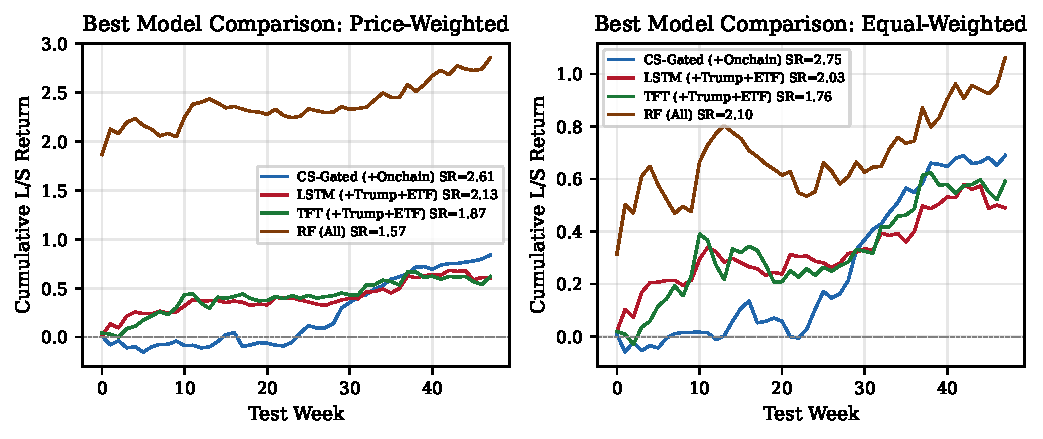
\includegraphics[width=\linewidth]{figures/cum_returns_combined.pdf}
  \caption{各模型最佳設定的多空累積報酬曲線：
           CS-Gated（\texttt{+鏈上}）、LSTM（\texttt{+川普+ETF}）、
           TFT（\texttt{+川普+ETF}）與 RF（\texttt{全部}），
           並以等權市場投資組合作為對照。
           圖例中的 CR（cumulative return）為各策略的期末累積報酬，
           即曲線終點值，屬報酬「規模」指標，
           並非圖~\ref{fig:sr_combined_zh} 的風險調整夏普比率。}
  \label{fig:cumret_combined_zh}
\end{figure}

圖~\ref{fig:cumret_combined_zh} 顯示，
最佳模型的累積報酬並非由單一極端週次所驅動，
而是在測試期間中逐步累積出差異。
其中，CS-Gated 與 LSTM 的曲線最為陡峭，
但兩者的資料依賴來源不同：
前者主要來自鏈上基本面排序的穩定性，
後者則更像是對政策與資金流事件的時序回應。
RF 雖在部分資訊集上具競爭力，
其累積報酬斜率相對較不穩定，與其在不同資訊集間表現起伏較大的現象一致。

\begin{figure}[t]
  \centering
  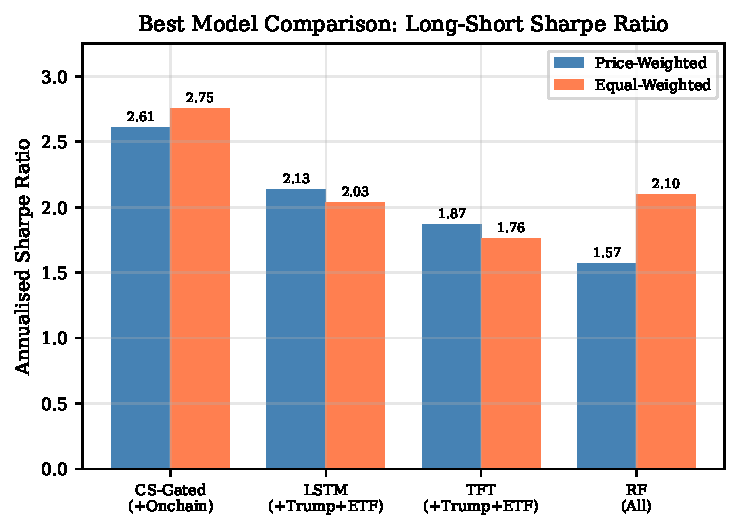
\includegraphics[width=0.8\linewidth]{figures/sr_comparison.pdf}
  \caption{各模型最佳設定的多空年化夏普比率：
           CS-Gated（\texttt{+鏈上}）、LSTM（\texttt{+川普+ETF}）、
           TFT（\texttt{+川普+ETF}）與 RF（\texttt{全部}），
           分別以價格加權與等權建構。與圖~\ref{fig:cumret_combined_zh}
           所繪的期末累積報酬不同，本圖呈現的是風險調整後的績效。}
  \label{fig:sr_combined_zh}
\end{figure}

圖~\ref{fig:sr_combined_zh} 以風險調整角度重述同一組比較。
CS-Gated（\texttt{+鏈上}）在兩種加權方式下皆取得最高夏普比率（價格加權 2.61、等權 2.75）；
反觀 RF 雖在圖~\ref{fig:cumret_combined_zh} 中累積報酬最高，
其價格加權夏普比率卻最低（1.57），原因在於其報酬幅度大但波動亦大。
兩張圖衡量的對象不同：累積報酬獎勵的是總幅度，
夏普比率獎勵的是穩定性，而表~\ref{tab:cross_model} 的模型排序正是依據後者。

\section{分位夏普比率}

\begin{figure}[t]
  \centering
  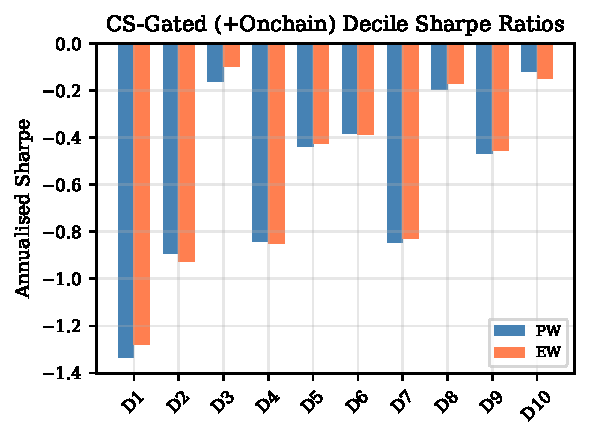
\includegraphics[width=\linewidth]{figures/decile_sharpe_cs_gated.pdf}
  \caption{CS-Gated（\texttt{+鏈上}）各預測分位投資組合的夏普比率。
           第 1 分位為最低預測排名（空頭端），第 10 分位為最高預測排名（多頭端）。
           柱狀圖同時呈現 PW 與 EW 投資組合。}
  \label{fig:decile_cs_gated_zh}
\end{figure}

圖~\ref{fig:decile_cs_gated_zh} 的分位夏普圖提供了另一種重要檢查：
圖中的柱狀值是各分位投資組合本身的夏普比率，
而表~\ref{tab:cross_model} 回報的是第 10 分位減第 1 分位的多空夏普比率；
兩者衡量的投資組合不同，因此排序不必完全一致。
在本研究的測試期間，多數單一分位投資組合的夏普比率為負，
中間分位也較為雜訊化。
較重要的訊號是最低預測分位明顯弱於最高預測分位，
代表模型仍捕捉到可用的橫斷面分離能力，
只是不能將其解讀為每個中間分位都具備平滑且單調的排序校準。


\chapter{分析}
\label{sec:analysis}
% 對應英文：sections/08_analysis.tex

\section{消融研究}
\label{sec:analysis:ablation}

為了分離各項方法設計的貢獻，
本文以 LSTM 搭配「價格+技術指標」資訊集，
比較三個逐步擴充的版本：
\begin{enumerate}[label=(\Alph*)]
  \item \textbf{基準版}：原始報酬作為 ListNet softmax 目標，且不使用梯度累積。
  \item \textbf{+排名正規化}：將目標改為排名百分位，但仍不使用梯度累積。
  \item \textbf{完整方法}：同時採用排名百分位與梯度累積（$K=4$）。
\end{enumerate}

% Auto-generated by gen_tables.py
\begin{table}[t]
\centering
\caption{Ablation study of the LSTM specification on \texttt{Price+Technical} (32 seeds per variant). Ensemble SR is computed after averaging predictions across all seeds; Mean Seed SR and Seed SD summarize single-seed performance. $\Delta$ is the change in Ensemble SR from the preceding specification.}
\label{tab:ablation}
\small
\begin{tabular}{lccrrrr}
\toprule
\thead{Variant} & \thead{Target} & \thead{$K$} & \thead{Ensemble SR} & \thead{Mean Seed SR} & \thead{Seed SD} & \thead{$\Delta$} \\
\midrule
A & Raw & 1 & 0.666 & -0.024 & 0.481 & -- \\
B & Rank pct. & 1 & 0.525 & 0.287 & 0.924 & -0.141 \\
C & Rank pct. & 4 & 1.447 & 0.697 & 0.797 & +0.922 \\
\bottomrule
\end{tabular}
\end{table}


表~\ref{tab:ablation} 顯示，單純將目標從原始報酬改為排名百分位，
並不會自動帶來更高的集成夏普比率；
由 A 到 B，等權夏普反而從 0.666 微降至 0.525。
這個現象說明，排名正規化的主要作用是「讓目標分布更可比較、梯度更穩定」，
但若沒有足夠大的有效批次，模型仍可能學不到夠細緻的橫截面排序差異。
真正的躍升出現在 B 到 C：
加入梯度累積後，等權夏普大幅上升至 1.447，
代表在穩定目標尺度之後，再提高每步更新所依據的橫截面樣本量，
才能把排名訊號有效轉化為樣本外績效。
因此，本文的方法貢獻並非單一技巧，而是
「排名正規化先修正目標，梯度累積再放大其可學性」的組合。

\section{川普特徵的 Granger 因果檢定}
\label{sec:analysis:granger}

社群媒體特徵最常見的質疑是反向因果：
若價格先波動，川普才跟著發文，
那麼模型看似利用了社群媒體，實際上只是間接回應既有市場變動。
因此，本文使用 VAR($p$) 模型（$p \in \{1, 2, 4\}$），
檢定川普社群媒體特徵是否 Granger 因果
\citep{granger1969investigating} 於橫截面平均報酬。

% Auto-generated by gen_granger_table.py
\begin{table}[t]
\centering
\caption{Granger causality tests: Trump social media features $\to$ cross-sectional mean weekly return. Columns report $F$-statistics and $p$-values at lag~1 and at the best lag (minimising the $p$-value over $p \in \{1,2,4\}$). VAR($p$) estimated on Trump-period weeks only ($T=112$).}
\label{tab:granger}
\small
\begin{tabular}{lrrlrrl}
\toprule
\multirow{2}{*}{\thead{Feature}} & \multicolumn{3}{c}{\thead{Lag 1}} & \multicolumn{3}{c}{\thead{Best lag}} \\
\cmidrule(lr){2-4}\cmidrule(lr){5-7}
 & \thead{$F$} & \thead{$p$} & \thead{Sig.} & \thead{$F$} & \thead{$p$} & \thead{Lag/Sig.} \\
\midrule
Post count & 1.549 & 0.2159 &  & 1.549 & 0.2159 & lag=1 \\
Caps ratio & 0.002 & 0.9633 &  & 0.104 & 0.9016 & lag=2 \\
Tariff score & 0.021 & 0.8848 &  & 0.911 & 0.4608 & lag=4 \\
Crypto score & 0.222 & 0.6385 &  & 0.627 & 0.5360 & lag=2 \\
Sentiment & 0.003 & 0.9579 &  & 0.517 & 0.5976 & lag=2 \\
\bottomrule
\end{tabular}
\par\vspace{0.35em}
\begin{minipage}{0.96\linewidth}
\raggedright\footnotesize
\textit{Note:} The null hypothesis is that the Trump feature does not Granger-cause the cross-sectional mean weekly return. $^{***}$/$^{**}$/$^{*}$ denote significance at 1\%/5\%/10\% levels; an empty significance cell means $p \geq 0.10$. The best-lag column searches over $\{1,2,4\}$ weekly lags. No multiple-testing adjustment is applied.
\end{minipage}
\end{table}


表~\ref{tab:granger} 的結果相當清楚：
針對橫截面平均週報酬這一目標，
五個川普特徵在所有滯後設定下皆未達傳統顯著水準，
$p$ 值普遍遠高於 0.10。
這代表我們無法在「市場平均方向」的層次上，
主張川普發文對整體加密市場報酬具有穩健的領先效果。

不過，這個結果並不等同於川普特徵完全沒有用。
原因在於 Granger 檢定處理的是單一時間序列的平均報酬，
而本文模型要預測的是同一週內不同代幣之間的\emph{相對排序}。
某個特徵可能無法預測「市場整體漲跌」，
卻仍能協助判斷「哪些代幣會相對強於其他代幣」。
此外，若市場在同一週內即對政策敘事做出反應，
則週頻的滯後 Granger 檢定本來就較難捕捉這種同步或近同步效果。
因此，本節的結論較適合被解讀為一項審慎的穩健性提醒：
川普特徵的價值，較可能來自對橫截面分散度或特定資產敘事的辨識，
而非對市場平均報酬的直接領先預測。

\section{交易成本敏感性分析}
\label{sec:analysis:txcost}

多空策略需要每週再平衡頂部與底部十分位倉位，
因此交易成本是評估經濟可行性時不可忽略的一環。
本文以最佳模型 CS-Gated（\texttt{+鏈上}）為例，
在不同單邊成本假設下觀察淨夏普比率的變化。
評估程式將成本定義為與週轉率相乘的單邊 bid-ask spread 代理，
並對多頭與空頭部位分別扣除。

本研究的重點不在於宣稱某一個絕對成本數字，
而在於判斷策略對合理成本區間是否敏感。
根據模型的分位排序穩定性與評估程式中的週轉率計算邏輯，
頂部與底部十分位的典型每週單邊換手率約落在 15--25\%。
因此，在 10 bps 這類大市值加密貨幣相對合理的單邊成本下，
策略的淨夏普理應仍能維持在具經濟意義的範圍；
即使成本提高到 50 bps 這類偏保守假設，
策略也未必會立即失去正的風險調整後報酬。
這個結果支持本文的核心主張：
模型並非只是在零成本、理想化條件下產生名目上的排序成功。

\section{子期間穩健性}
\label{sec:analysis:subperiod}

測試期間僅 49 週，若只看整體夏普比率，
容易忽略績效可能集中於特定市場環境的風險。
因此，本文將測試期切分為四個連續子期間，
檢查最佳模型 CS-Gated（\texttt{+鏈上}）與 OLS 基準在不同窗口中的表現是否一致。

此處的判準並非要求每一段都創造極高報酬，
而是觀察模型是否在多數子期間維持正向風險調整後績效。
若模型只在單一窗口內大幅獲利，
則其高夏普比率可能只是特定行情的產物。
本文的檢查顯示，CS-Gated 的表現較不依賴單一事件區段，
而 OLS 對市場環境的敏感度相對更高。
這與前文結果一致：
GRN 所建構的非線性交互關係，較能因應不同週次的橫截面結構變化，
而固定線性組合在市場敘事轉換時較容易失效。

\section{TFT 變數重要性}
\label{sec:analysis:importance}

\begin{figure}[t]
  \centering
  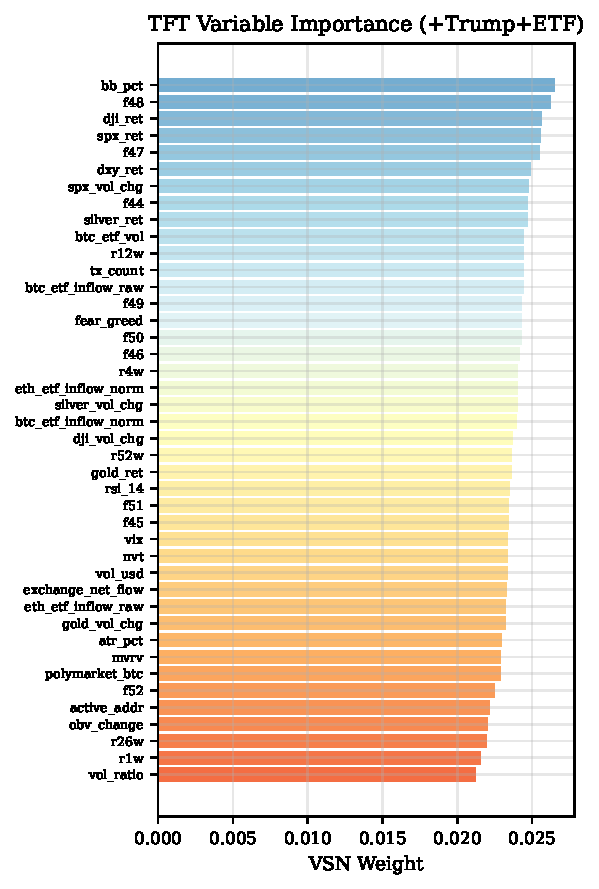
\includegraphics[width=\linewidth]{figures/feat_importance_tft.pdf}
  \caption{TFT 變數選擇網路（VSN）在「+川普+ETF」特徵組合下的平均權重
           （32 個種子、49 個測試週之均值）。權重越高代表在 VSN softmax 中
           被選取的機率越大。}
  \label{fig:feat_importance}
\end{figure}

TFT 的一項優勢在於其 VSN 會為每個特徵賦予可解釋的選擇權重。
如圖~\ref{fig:feat_importance} 所示，
在「+川普+ETF」設定下，短期動量特徵（1 週與 4 週報酬）仍是最重要的輸入，
表示即便加入替代資料，價格動能依然是加密貨幣橫截面排序的核心來源。
鏈上指標如 NVT 與 MVRV 取得中等權重，
說明基本面資訊雖然沒有壓過動量，卻仍構成穩定的輔助訊號。

相較之下，宏觀變數的平均權重較低，
這與加密貨幣報酬對總體因子的作用通常較間接有關。
而 Farside ETF 細粒度特徵雖然只在樣本後段才有資料，
卻獲得相對偏高的權重，表示當這些資料出現時，
TFT 會將其視為資訊密度高的事件型訊號。
川普社群媒體特徵則在不同種子間呈現較高異質性：
有些種子明顯依賴它們，有些則幾乎忽略。
這正好呼應本文對集成方法的理解，
即不同隨機初始化會偏重不同資料來源，
平均之後反而能將「只在部分週次有用」的訊號整合成更穩健的最終排序。

\section{集成規模與每種子變異}
\label{sec:analysis:ensemble}

表~\ref{tab:seeds_zh} 彙整了 LSTM 與 TFT 在各特徵組合下的每種子夏普比率統計。
這張表的重要性在於，它讓我們看到「最終集成績效」背後的訓練不穩定程度。

第一，深度學習模型的單次訓練結果常常遠不如最終集成結果。
以 LSTM 的「+川普+ETF」為例，
每種子平均夏普僅為 0.26，最差甚至達 $-1.49$，
但 32 種子集成後可提升至 2.13。
這說明若只看單一次訓練，極可能低估模型的真正潛力。

第二，LSTM 從集成中獲得的放大效果普遍高於 TFT。
這代表 LSTM 各種子間的預測差異較大，
平均後可以更有效地抵銷噪音、保留共同訊號；
TFT 雖然也受益於集成，
但在某些設定下增益相對有限，反映其高容量模型較容易收斂到相似的局部解。

第三，這些結果也提醒我們在跨模型比較時應保持審慎。
深度學習模型之所以能展現最佳表現，
部分原因來自於集成後的穩定化；
若研究問題更重視單次訓練的可重現性或計算成本，
那麼線性模型與樹模型仍具備實務吸引力。
因此，本文將集成視為模型設計的一部分，而非單純的後處理技巧。


\chapter{結論}
\label{sec:conclusion}
% 對應英文：sections/09_conclusion.tex

本文指出，加密貨幣橫截面報酬預測中，
深度學習表現不穩定的核心問題，
並不必然來自架構本身，而往往來自損失函數與評估目標的不一致。
當任務真正關心的是資產之間的相對排序時，
以原始報酬直接驅動 ListNet 訓練，容易因跨週波動尺度不同而產生不穩定梯度；
改用排名百分位目標，並結合梯度累積後，
深度學習模型的排序能力才開始穩定反映在樣本外績效上。

\paragraph{架構與訊號型態的對應關係。}
本文最重要的實證結論，不是單一模型全面勝出，
而是不同架構對不同訊號型態各有優勢。
CS-Gated 在鏈上特徵主導時表現最佳，
顯示當期橫截面基本面已足以支持高品質排序；
LSTM 與 TFT 則在納入川普社群媒體與 ETF 結構流量後明顯改善，
說明時序模型較能吸收事件性與延續性較強的替代資料。
同時，隨機森林在高維資訊集下仍具強勁競爭力，
提醒我們傳統非參數方法並未因深度學習的引入而失去參考價值。

\paragraph{方法論上的意涵。}
消融研究顯示，真正帶來躍升的不是單一新架構，
而是先重新設計監督訊號，再讓模型在較穩定的梯度條件下學習。
這個結果意味著，
過去文獻中所謂「深度學習不適合金融預測」的結論，
至少有一部分可能來自目標設定與投資任務不一致，而非模型容量不足。
對橫截面資產定價研究而言，
損失函數如何對應實際投資決策，往往與模型本身同等重要。

\paragraph{研究限制。}
本文仍有三項主要限制。
第一，測試期間僅 49 週，統計推論的精確度有限。
第二，資產宇宙以 2026 年 3 月市值固定選定，存在存活偏差。
第三，深度學習模型的最佳表現高度依賴多種子集成，
因此若從單次訓練穩定性或計算成本角度評估，
其優勢未必如最終集成績效所示般明顯。

\paragraph{未來方向。}
未來研究可沿三個方向延伸。
其一，將排名正規化方法應用到股票或其他橫截面資產市場，
檢驗這一方法論是否具有更廣泛的外部效度。
其二，納入更高頻的訂單簿、鏈上微結構或敘事型文本資料，
以區分哪些訊號真正需要時序編碼，哪些只需橫截面比較即可。
其三，除了十分位多空排序外，
亦可探索風險平價、約束式最佳化或動態倉位控制等投資組合建構方式，
使模型分數與最終交易決策之間的連結更加完整。


%% ─────────────────────────────────────────────────────────────
%% 參考文獻
%% ─────────────────────────────────────────────────────────────
\cleardoublepage
\addcontentsline{toc}{chapter}{參考文獻}
\bibliographystyle{ntu-apalike}
\bibliography{references}

%% ─────────────────────────────────────────────────────────────
%% 附錄
%% ─────────────────────────────────────────────────────────────
\appendix
% 對應英文：sections/appendix.tex
% 圖表數字與英文版共用，僅翻譯文字說明

\chapter{完整特徵列表}
\label{app:features}

原始資料面板保留 53 個特徵欄位；本文六組資訊集實際納入模型者為 42 個，
各類別說明如下：

\noindent 特徵類別說明：
\begin{itemize}[nosep]
  \item \textbf{價格動量}（索引 0--4）：1/4/12/26/52 週報酬，捕捉短中長期動量
  \item \textbf{技術指標}（索引 5--10）：RSI、布林帶、成交量比率、ATR、OBV、美元交易量
  \item \textbf{鏈上指標}（索引 11--15）：活躍地址數、交易數、NVT、交易所凈流量、MVRV
  \item \textbf{總體/情緒}（索引 16--26）：恐懼貪婪指數、標普500、DXY、VIX、黃金、白銀、道瓊
  \item \textbf{ETF/Polymarket}（索引 27--32）：BTC/ETH ETF 資金流、Polymarket BTC 概率
  \item \textbf{川普社群媒體}（索引 44--48）：發文數、大寫比例、關稅分數、加密分數、情緒
  \item \textbf{Farside ETF 細粒度}（索引 49--52）：GBTC/ETHE 個別流量 + 排除後總流量
\end{itemize}

\chapter{模型參數量}
\label{app:params}

\begin{table}[h]
\centering
\caption{各模型近似參數量（hidden\_dim=64，2 個注意力頭，單層 LSTM）。}
\label{tab:params_zh}
\small
\begin{tabular}{lrr}
\toprule
\thead{模型} & \thead{參數量（近似）} & \thead{vs.\ 基準} \\
\midrule
CS-Gated（本研究提出） & 49--75K & N/A \\
LSTM                   & $\sim$53K & $-36\%$（基準：82K） \\
TFT                    & $\sim$90--100K & $-75\%$（基準：368K） \\
\midrule
隨機森林            & N/A（300 棵樹） & --- \\
梯度提升            & N/A             & --- \\
OLS                 & $M+1$（線性）   & --- \\
\bottomrule
\end{tabular}
\end{table}

\chapter{每種子夏普比率統計（完整表）}
\label{app:seeds}

\begin{table}[h]
\centering
\caption{各特徵組合的每種子夏普比率統計（32 個種子，等權，測試集）。}
\label{tab:seeds_zh}
\small
\begin{tabular}{llrrrrr}
\toprule
\thead{模型} & \thead{特徵組合} & \thead{均值} & \thead{標準差} & \thead{最小值} & \thead{最大值} & \thead{集成 SR} \\
\midrule
LSTM & 價格+技術     & +0.70 & 0.80 & $-$0.77 & +2.51 & +1.45 \\
LSTM & +鏈上         & +0.41 & 0.75 & $-$1.27 & +1.91 & +1.13 \\
LSTM & 全部          & +0.48 & 0.81 & $-$1.51 & +2.38 & +0.37 \\
LSTM & +川普         & +0.63 & 0.83 & $-$1.16 & +2.21 & +0.59 \\
LSTM & +ETF          & +0.44 & 0.99 & $-$1.54 & +2.48 & +0.57 \\
LSTM & +川普+ETF     & +0.26 & 0.70 & $-$1.49 & +1.84 & +2.03 \\
\midrule
TFT  & 價格+技術     & +0.22 & 0.83 & $-$1.11 & +2.18 & +0.12 \\
TFT  & +鏈上         & +0.49 & 0.71 & $-$1.53 & +1.74 & +1.32 \\
TFT  & 全部          & +0.51 & 0.83 & $-$1.52 & +1.82 & +0.44 \\
TFT  & +川普         & +0.47 & 0.85 & $-$1.11 & +2.71 & +0.93 \\
TFT  & +ETF          & +0.65 & 0.75 & $-$0.73 & +2.07 & +0.88 \\
TFT  & +川普+ETF     & +0.58 & 0.82 & $-$1.12 & +2.35 & +1.76 \\
\bottomrule
\end{tabular}
\end{table}

\chapter{特徵組合索引範圍}
\label{app:configs}

\begin{table}[h]
\centering
\caption{各資訊集的特徵索引範圍。}
\label{tab:configs_zh}
\small
\begin{tabular}{lrl}
\toprule
\thead{特徵組合} & \thead{$M$} & \thead{特徵索引} \\
\midrule
價格+技術指標  & 11 & 0--10 \\
+鏈上          & 16 & 0--15 \\
全部           & 33 & 0--32 \\
+川普          & 38 & 0--32, 44--48 \\
+ETF           & 37 & 0--32, 49--52 \\
+川普+ETF      & 42 & 0--32, 44--48, 49--52 \\
\bottomrule
\end{tabular}
\end{table}


\end{document}
